
%for compiling, enter
%pdflatex main_doc.tex & bibtex main_doc.aux & pdflatex main_doc.tex & pdflatex main_doc.tex

\documentclass[a4paper]{jpconf}
\bibliographystyle{iopart-num}
\usepackage{citesort}
\usepackage{amsmath}
%% \usepackage[square,sort&compress]{natbib}

\newcommand{\REVTeX}{REV\TeX}

\sloppy 

\usepackage{graphicx}
\begin{document}
\title{Prediction of uncertainty of 10-coefficient compressor maps for extreme operating conditions}

\author{Howard Cheung}

\address{Postdoctoral Research Fellow, Ray W. Herrick Laboratories, School of Mechanical Engineering, Purdue University, 177 S. Russell St., West Lafayette, IN 47907-2031, US}

\ead{cheung@purdue.edu}

\author{Christian K. Bach}

\address{Assistant Professor, Mechanical and Aerospace Engineering, Oklahoma State University, 218 Engineering North, Stillwater, OK 74078-5016}

\ead{cbach@okstate.edu}

\begin{abstract}
Empirical compressor maps are a simple and reliable approach for heating and cooling system designers to estimate compressor refrigerant mass flow rate and power consumption quickly. These maps were used for a long time since most compressor manufacturers build the maps with extensive test matrices, leading to good accuracy. However, the situation changes when engineers extrapolate the maps to investigate the compressor��s performance under extreme operating conditions such as for cold climate heat pump applications or under conditions with system faults.  Engineers are not confident on the exact uncertainty of the extrapolation, and often claim that the inaccuracy of their studies is a result of high extrapolation uncertainty. This paper presents a method to estimate the extrapolation uncertainty due to the structure of the test matrix that trains the manufacturer maps and helps the investigators to understand if the extrapolation is the main cause of their inaccuracy. To verify that the method can estimate the uncertainty due to extrapolation, the study builds 10-coefficient compressor maps trained by different test matrices of the same size and different operating points. The maps are used to estimate the compressor performance under different operating points and their estimation uncertainties are compared. The results show that the component of the uncertainty that depends on the structure of the test matrix is small at operating conditions within the test matrix but the uncertainty grows significantly as the estimation becomes further away from the operating conditions within the test matrices.
\end{abstract}

\section{Sources of uncertainty} \label{sec:sources}
\label{sec:uncer_source}

Uncertainty of the compressor map output is the range where the true value of the output may be relative to the map output. It consists of multiple components and can be grouped as follows:

\begin{itemize}
\item Uncertainty due to inputs
\item Uncertainty due to training data
\item Uncertainty due ot model random error
\item Uncertainty due to outputs
\end{itemize}

\subsection{Uncertainty due to inputs} \label{subsec:uncer_inputs}
Uncertainty due to inputs is the uncertainty propagated to the map output due to the uncertainty in the inputs to the maps. The inputs to the map (evaporating and condenser temperature) are usually obtained by converting pressure measurements to saturation temperatures with refrigerant equations of state. Therefore the estimated saturation temperature contains uncertainty from both the equation of state and the pressure measurement. The equation of state of R22 estimates saturation pressure at an uncertainty of 0.2\% \cite{Kamei:1995}. When the equation of state estimates an saturation temperature at a given pressure, this uncertainty is transformed into a component of the uncertainty of the saturation temperature as shown in

\begin{equation}
\frac{\Delta P_{sat,EOS}}{P_{sat}(T)} = 0.2\% = 0.002
\label{eq:uncer_p_eos}
\end{equation}

and

\begin{equation}
\Delta {T_{sat,EOS}} = \left|{\frac{{\partial {T_{sat}}({P})}}{{\partial {P}}}}\right|\Delta {P_{sat,EOS}} ,
\label{eq:uncer_t_eos}
\end{equation}

where $\Delta P_{sat,EOS}$ is the uncertainty of saturation pressure as a result of uncertainty of the equation of state, $P_{sat}(T)$ is the saturation pressure from temperature $T$, $\Delta {T_{sat,EOS}}$ is the uncertainty of saturation temperature as a result of uncertainty of the equation of state and ${T_{sat}}({P})$ is the saturation temperature at pressure $P$.

The component of the saturation temperature uncertainty due to pressure measurement is calculated by

\begin{equation}
\Delta {T_{sat,mea}} = \left|\frac{{\partial {T_{sat}}({P})}}{{\partial {P}}}\right|\Delta {P_{sat,mea}},
\label{eq:uncer_t_mea}
\end{equation}

where $\Delta {T_{sat,mea}}$ is the uncertainty of saturation temperature as a result of pressure measurement and $\Delta P_{sat,mea}$ is the uncertainty of pressure measurement. The overall uncertainty of the saturation temperature is given by 

\begin{equation}
\Delta {T_{sat}} = \sqrt {{{(\Delta {T_{sat,EOS}})}^2} + {{(\Delta {T_{sat,mea}})}^2}} .
\label{eq:uncer_t}
\end{equation}

The uncertainty of the map output propagated from the inputs of condensing temperature and evaporating temperature is calculated by

\begin{equation}
\Delta {\hat{\dot{W}}_{input}} = \sqrt {{\left(\frac{{\partial \hat{\dot{W}}}}{{\partial {T_{evap}}}}\Delta {T_{evap}}\right)^2} + {\left(\frac{{\partial \hat{\dot{W}}}}{{\partial {T_{cond}}}}\Delta {T_{cond}}\right)^2}}, 
\label{eq:uncer_w_input}
\end{equation}

where $\Delta {\hat{\dot{W}}_{input}}$ is the uncertainty due to inputs at the map output, $\Delta {T_{evap}}$ is the uncertainty of evaporating temperature at input and $\Delta T_{cond}$ is the uncertainty of condensing temperature at input

\subsection{Uncertainty due to training data} \label{subsec:uncer_train}
Uncertainty due to training data is the uncertainty propagated to the map output from the training data through the map coefficients. This can be understood by considering the estimation of the map coefficients as a function of the training data as

\begin{equation}
\hat{ \vec {\beta}}  = g({T_{evap,train,1}},...,{T_{evap,train,n}},{T_{cond,train,1}},...,{T_{cond,train,n}},{\dot{W}_{train,1}},...,{\dot{W}_{train,n}}), 
\label{eq:beta_train}
\end{equation}

where n is the number of training data points. Through function $g$ and $\hat{ \vec {\beta}}$ in Eqn. (\ref{eq:beta_train}), as suggested in \cite{song:2013}, the uncertainty component due to training data is calculated

\begin{equation}
\Delta {\hat{\dot{W}}_{train}} = \sqrt{\begin{gathered}
  \Sigma_{j=1}^n\left(\Sigma _{i = 1}^m\left(\frac{{\partial \hat{\dot{W}}}}{{\partial {\beta _i}}}\frac{{\partial {\beta _i}}}{{\partial {T_{evap,train,j}}}}\right)\Delta {T_{evap,train,j}}\right)^2  \hfill \\
  +\Sigma_{j=1}^n\left(\Sigma _{i = 1}^m\left(\frac{{\partial \hat{\dot{W}}}}{{\partial {\beta _i}}}\frac{{\partial {\beta _i}}}{{\partial {T_{cond,train,j}}}}\right)\Delta {T_{cond,train,j}}\right)^2 \hfill \\
   +\Sigma_{j=1}^n\left(\Sigma _{i = 1}^m\left(\frac{{\partial \hat{\dot{W}}}}{{\partial {\beta _i}}}\frac{{\partial {\beta _i}}}{{\partial {\dot{W}_{,train,j}}}}\right)\Delta {\dot{W}_{train,j}}\right)^2 \hfill \\ 
\end{gathered}}, 
\label{eq:uncer_w_train}
\end{equation}

where $\Delta {\hat{\dot{W}}_{train}}$ is the uncertainty due to training data at the map output, $\Delta {T_{evap,train,j}}$ is the uncertainty of the evaporating temperature at the j$^{th}$ data point, $\Delta {T_{cond,train,j}}$ is the uncertainty of the condensing temperature at the j$^{th}$ data point, $\Delta {\dot{W}_{train,j}}$ is the uncertainty of the power consumption at the j$^{th}$ data point, and m is the number of coefficients in $\hat{\vec{\beta}}$.

\subsection{Uncertainty due to model random error} \label{subsec:uncer_model}

In linear regression, the random error between true model and actual system, $\varepsilon$ in Eqn. (\ref{eq:true_lin_model}) is assumed to be normally distributed around zero with some finite variance. This variance becomes part of the uncertainty of the uncertainty of the map output and can be presented in the form of confidence intervals. Statistic textbooks \cite{Montgomery:2005,Graybill:1994} illustrated that the confidence interval of the variance can be calculated as

\begin{equation}
\Delta {\hat{\dot{W}}_{model}} = {t_{n - m,1 - \alpha /2}}\sigma \sqrt {1 + {{\vec x}^T}{{({\mathbf{X}}_{train}^T{{\mathbf{X}}_{train}})}^{ - 1}}\vec x}
\label{eq:uncer_w_model}
\end{equation}

where $\Delta {\hat{\dot{W}}_{train}}$ is the uncertainty due to model random error at the map output.

One significant term in Eqn. (\ref{eq:uncer_w_model}) is ${\vec x^T}{({\mathbf{X}}_{train}^T{{\mathbf{X}}_{train}})^{ - 1}}\vec x$ which is the leverage of a regression model \cite{Atkinson:1987}. It estimates how deviated the current input vector to the map is relative to the training data of the regression model, and the magnitude of the leverage grows with the deviation. This helps to understand if the estimation is related to the training data and if (or ``how much'')the model is applicable at the current situation described by the input vector.

\subsection{Uncertainty due to output} \label{subsec:uncer_output}

Uncertainty of the map output should represent the probable range where the true value lies relative to the map output. However, since the map is built from data obtained from measured power consumption instead of true values of the power consumption, the uncertainty components of the map output propagated from other sources only estimate the uncertainty of the estimation with the measured power consumption. Another component of uncertainty must be introduced so that the map output uncertainty is the uncertainty to the true map output. This uncertainty component can be approximated with the uncertainty of the measured power consumption with its true values by

\begin{equation}
\Delta {\hat{\dot{W}}_{output}} = \frac{1}{n}\Sigma _{i = 1}^n\frac{{\Delta {{\dot{W}}_{train,i}}}}{{{{\dot{W}}_{train,i}}}} .
\label{eq:uncer_w_output}
\end{equation}

\subsection{Overall uncertainty} \label{subsec:overall_uncer}

The overall uncertainty of the map output is given by the square of the sum of all uncertainty components as

\begin{equation}
\Delta \hat{\dot{W}}= \sqrt {{{(\Delta {{\hat{\dot{W}}}_{input}})}^2} + {{(\Delta {{\hat{\dot{W}}}_{train}})}^2} + {{(\Delta {{\hat{\dot{W}}}_{model}})}^2} + {{(\Delta {{\hat{\dot{W}}}_{output}})}^2}} .
\label{eq:overall_uncer}
\end{equation}

\subsection{Effect of range of training data on map output} \label{subsec:comp_uncer}

To study how the range of training data affects the extrapolation uncertainty and accuracy, the difference between the map output and approximated measurement and the map output uncertainty for all data points in Figure \ref{fig:oper_envelope} are plotted in Figure \ref{fig:rel_uncer}, and a similar figure with their uncertainty components is plotted in Figure \ref{fig:uncer_comp}.

\begin{figure}[h]
\begin{minipage}{15pc}
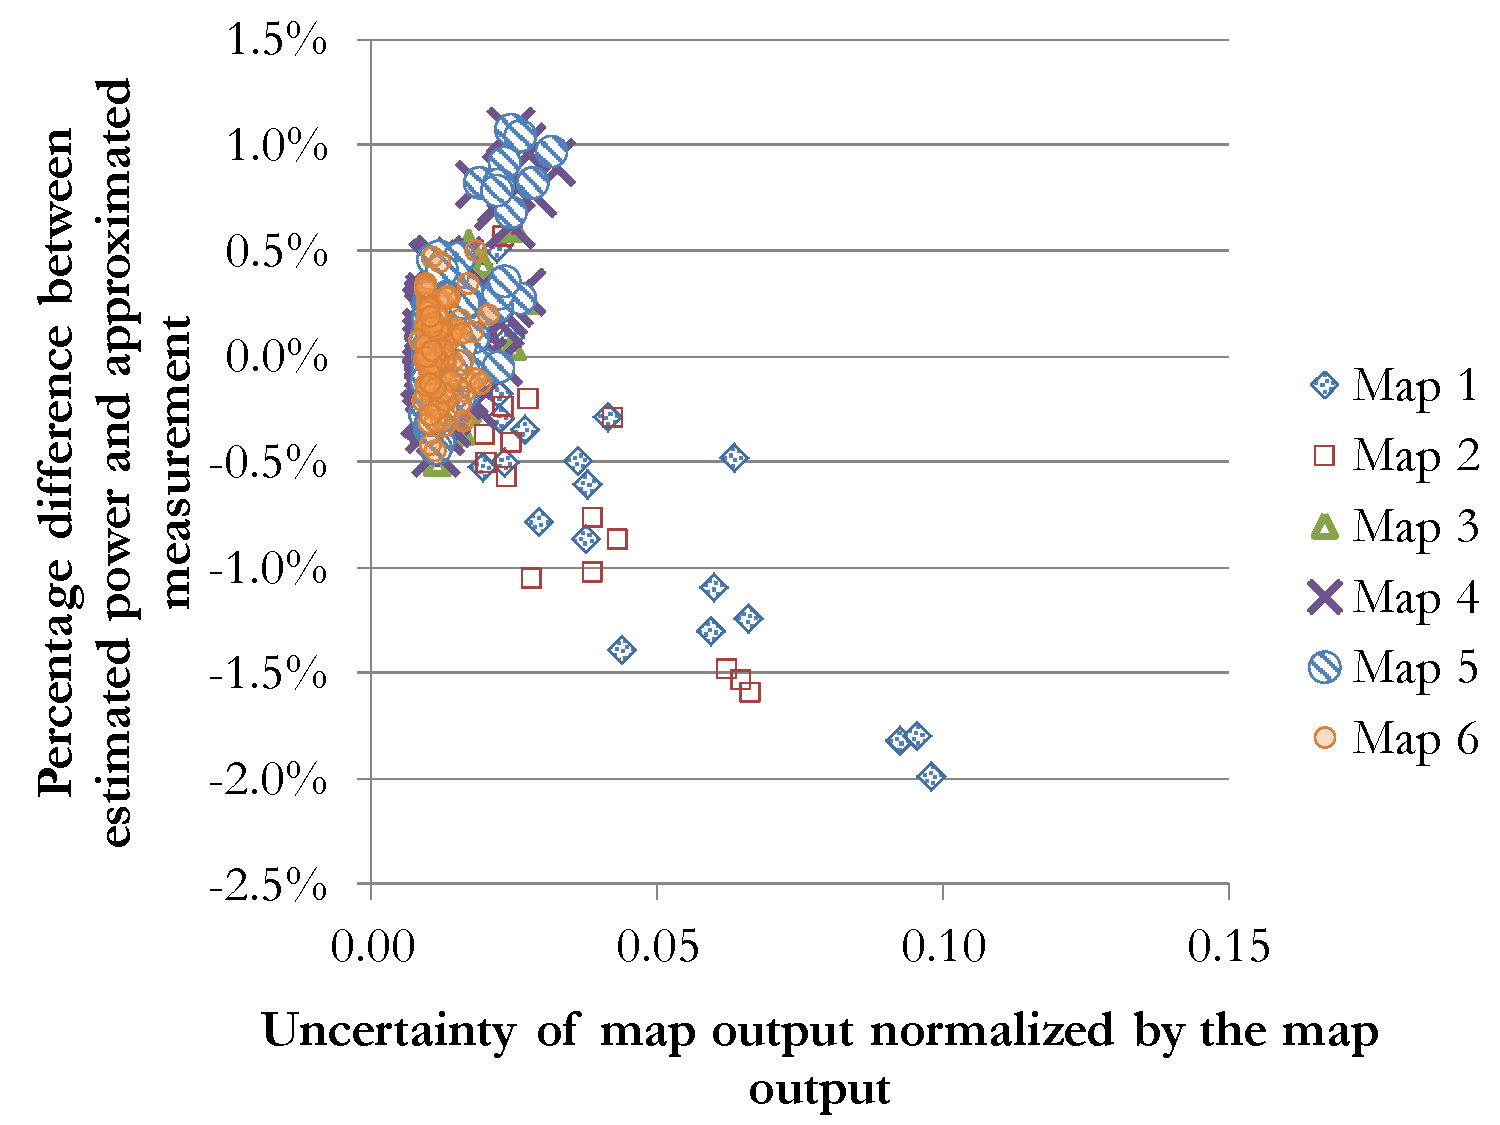
\includegraphics[width=15pc]{rel_diff_to_rel_uncer.pdf}
\caption{\label{fig:rel_uncer}Change of accuracy of maps with output uncertainty in different maps.}
\end{minipage}\hspace{2pc}%
\begin{minipage}{15pc}
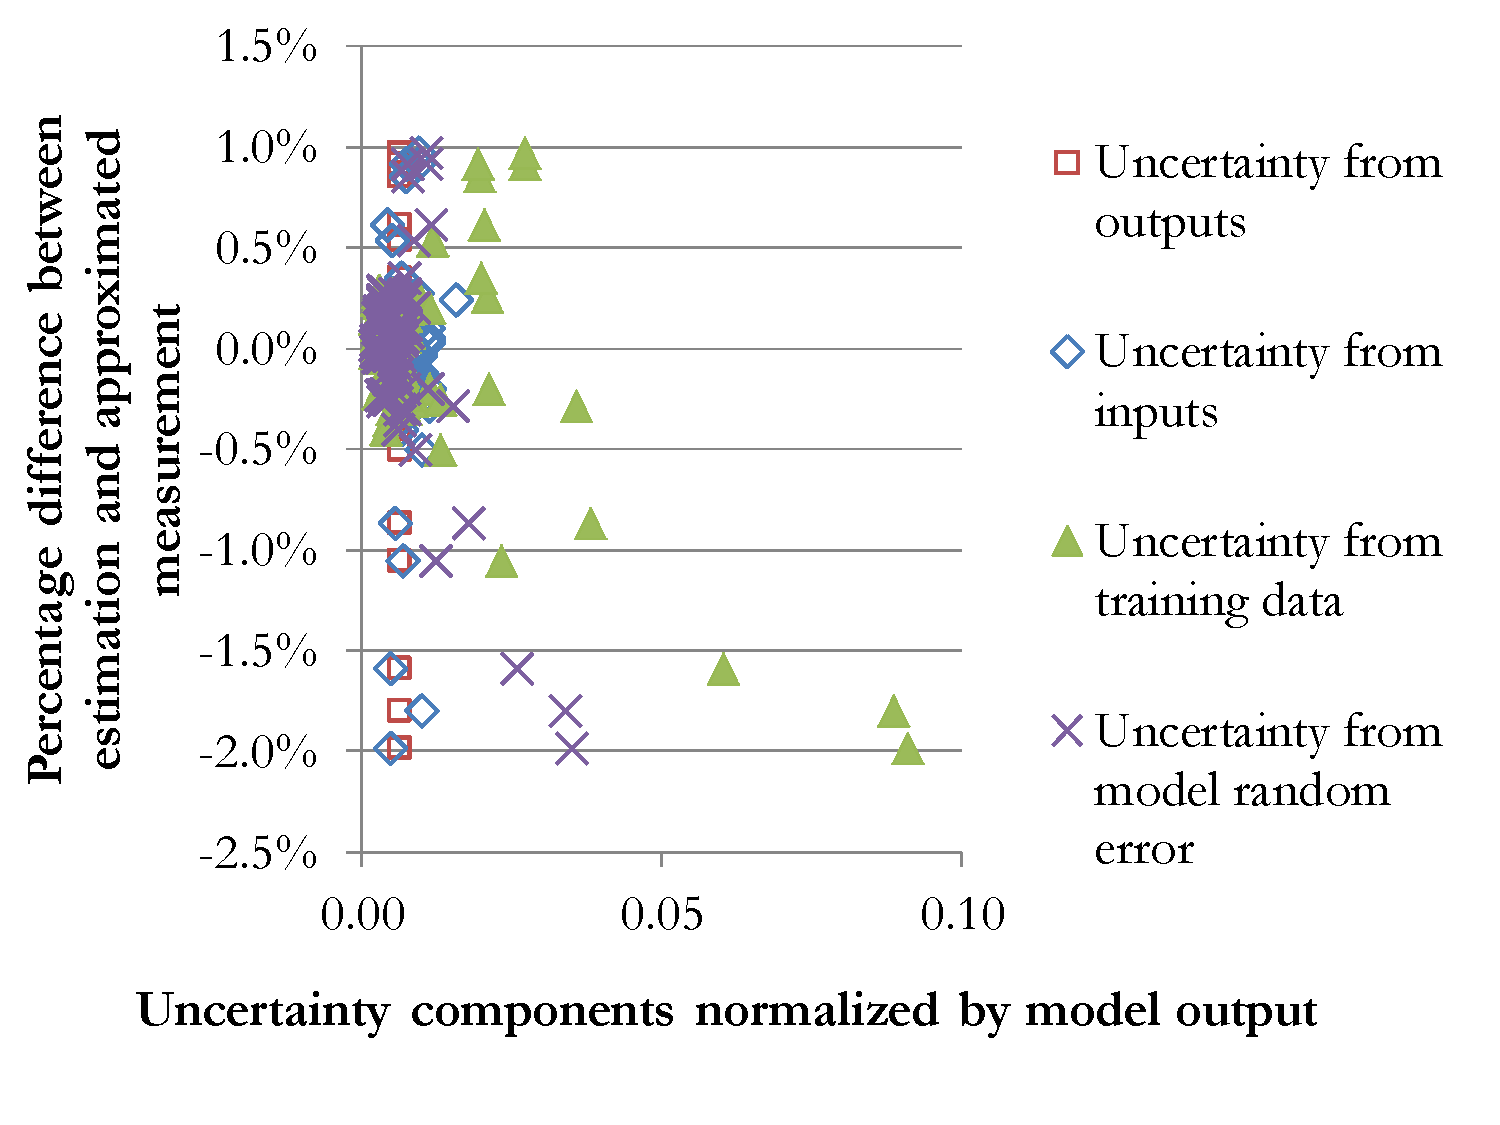
\includegraphics[width=15pc]{rel_diff_to_uncer_comp.pdf}
\caption{\label{fig:uncer_comp}Change of accuracy of maps with different uncertainty components.}
\end{minipage} 
\end{figure}

Figure \ref{fig:rel_uncer} shows that inaccurate map outputs are associated with higher uncertainty and the uncertainty calculation method is a good indicator of the accuracy of the map output. Figure \ref{fig:uncer_comp} shows that the high uncertainty of the inaccurate data points in Figure \ref{fig:rel_uncer} are primarily a result of high uncertainty from model random error and training data.

The increase of uncertainty from model random error with inaccuracy can be explained by the leverage term ${\vec x^T}{({\mathbf{X}}_{train}^T{{\mathbf{X}}_{train}})^{ - 1}}\vec x$ in Eqn. (\ref{eq:uncer_w_model}) which increases as the map extrapolates, and map extrapolation results in lower accuracy. Hence the uncertainty from model random error increase with a decrease of the map accuracy and applicability.

To explain the increase of uncertainty from training data with a decrease of map accuracy in Figure \ref{fig:uncer_comp}, the squared terms in Eqn. (\ref{eq:uncer_w_train}) are labeled as uncertainty from training data per measurement, and their values from two map outputs of Map 1 are plotted as Figures \ref{fig:map_1_low_uncer} and \ref{fig:map_1_high_uncer}.

\begin{figure}[h]
\begin{minipage}{15pc}
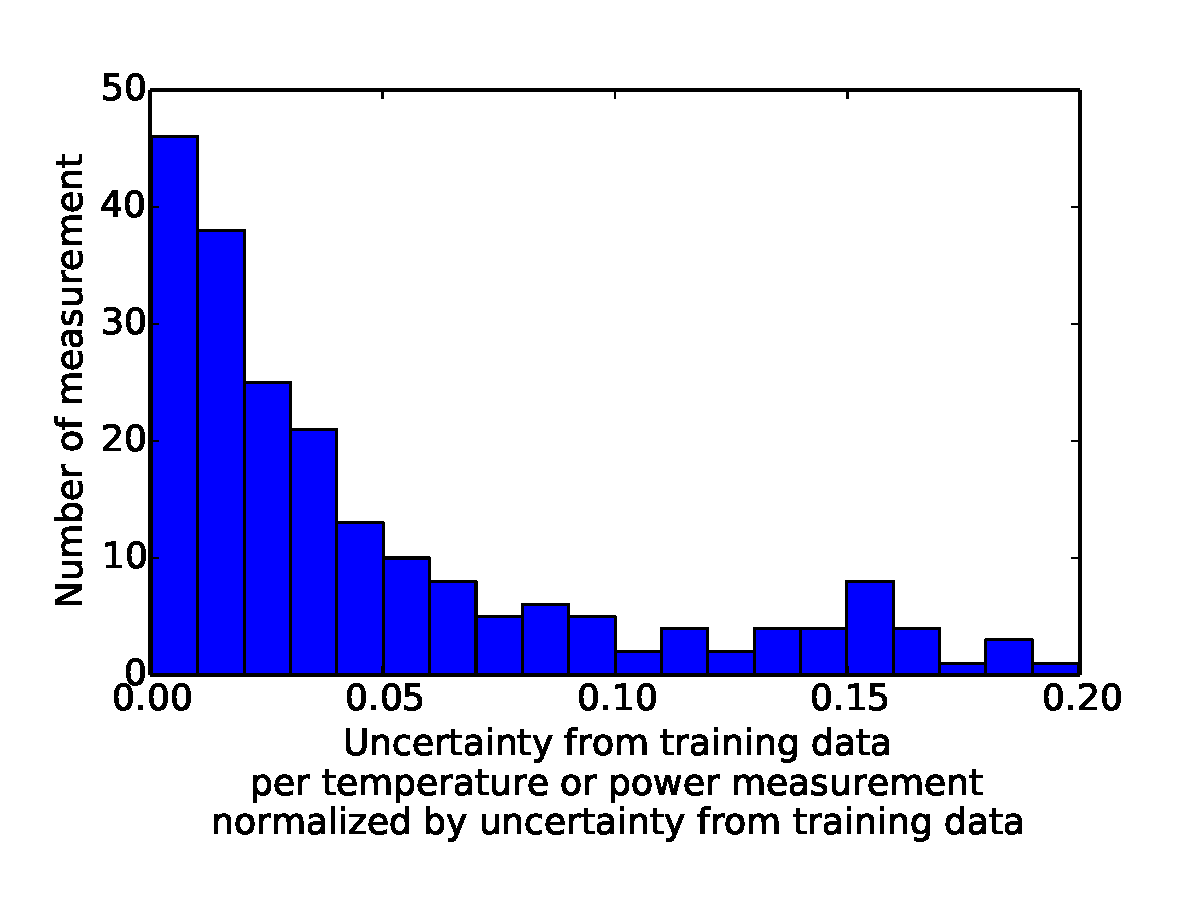
\includegraphics[width=15pc]{Map_1_low_uncer.pdf}
\caption{\label{fig:map_1_low_uncer}Histogram of uncertainty terms in Eqn. (\ref{eq:uncer_w_train}) for $T_{evap} = -1.1^\circ C$ and $T_{cond} = 60.0^\circ C$.}
\end{minipage}\hspace{2pc}%
\begin{minipage}{15pc}
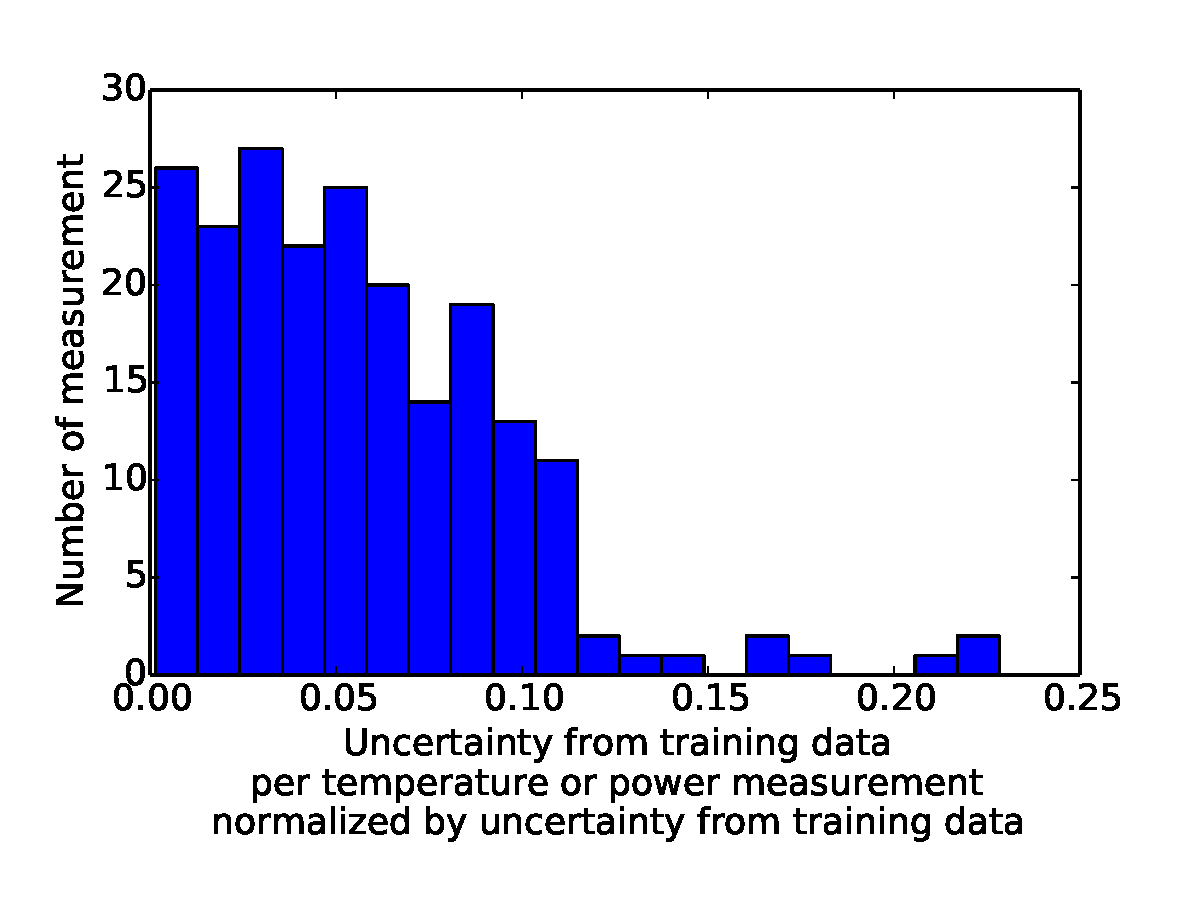
\includegraphics[width=15pc]{Map_1_high_uncer.pdf}
\caption{\label{fig:map_1_high_uncer}Histogram of uncertainty terms in Eqn. (\ref{eq:uncer_w_train}) for $T_{evap} = -28.9^\circ C$ and $T_{cond} = 26.7^\circ C$.}
\end{minipage} 
\end{figure}

Figure \ref{fig:map_1_low_uncer} shows a histogram that is more left-skewed than Figure \ref{fig:map_1_high_uncer}. This is because Figure \ref{fig:map_1_low_uncer} is obtained from a data point inside the training data range of Map 1 (see Figure~\ref{fig:training_envelope}), and the map only needs information from a few data points around $T_{evap} = -1.1^\circ C$ and $T_{cond} = 60.0^\circ C$ to estimate its map output. Hence the estimation does not depend on most of the data points, and their training data uncertainties do not propagate to the map output as shown by Figure \ref{fig:map_1_low_uncer}. 

However, Map 1 extrapolates to the lower left handed corner in Figure \ref{fig:training_envelope} for the condition in Figure \ref{fig:map_1_high_uncer}, and the estimation is significantly affected by multiple data points in the training data. If any of these significant training data points change, the estimation result at this condition will be changed significantly. Hence much more training data points propagate their uncertainty to the map output under the condition in Figure \ref{fig:map_1_high_uncer} than that in Figure \ref{fig:map_1_low_uncer}. This also explains that the uncertainty of training data is a significant component in the extrapolation uncertainty of the map output, and the uncertainty increases as the map applicability and accuracy decrease.


\subsection{Effect of number of training data points on map output} \label{subsec:num_train}

To understand how the number of training data points affect the map output, another map (Map 7) was created with the same range of training data as Map 1 and 24 data points only, as shown in Figure \ref{fig:map_1_7_training_data}. The accuracy of Map 7, rated by coefficient of variation $cov$ as 

\begin{equation}
cov = \frac{\text{Sum of squares of errors}}{\text{Mean value of estimated values}} = \frac{\text{Sample standard deviation}}{\text{Mean value of estimated values}} = \frac{\sigma}{1/n\cdot\Sigma_1^n \hat{y}_i}
\label{eq:cov}
\end{equation}
\blCom{changed above formula, please double-check if correct}
is compared with that of Map 1 in Table \ref{tb:map7_acc}.

\begin{table}[h]
\caption{\label{tb:map7_acc}Accuracy of Maps 1 and 7.}
\begin{center}
\begin{tabular}{p{1.2cm} p{6cm} p{5.7cm}}
\br
Map & Coefficient of variation based on training data poinst only ($cov_{train}$) & Coefficient of variation based on all data points in Figure \ref{fig:oper_envelope} ($cov_{all}$) \\
\mr
Map 1&0.18\%&0.31\%\\
Map 7&0.17\%&1.10\%\\
\br
\end{tabular}
\end{center}
\end{table}

Table \ref{tb:map7_acc} shows that the accuracy of Map 7 is similar to that of Map 1 at the training data points, but the analysis with all available data points shows that Map 7 is less accurate than Map 1. This shows that using fewer training data points reduces map accuracy. But to know if the reduction of accuracy happens at extrapolation, the accuracy of the map outputs is compared with the uncertainty from model random error and the uncertainty from training data as shown in Figures \ref{fig:num_train_model} and \ref{fig:num_train_train}.

\begin{figure}[h]
\begin{minipage}{15pc}
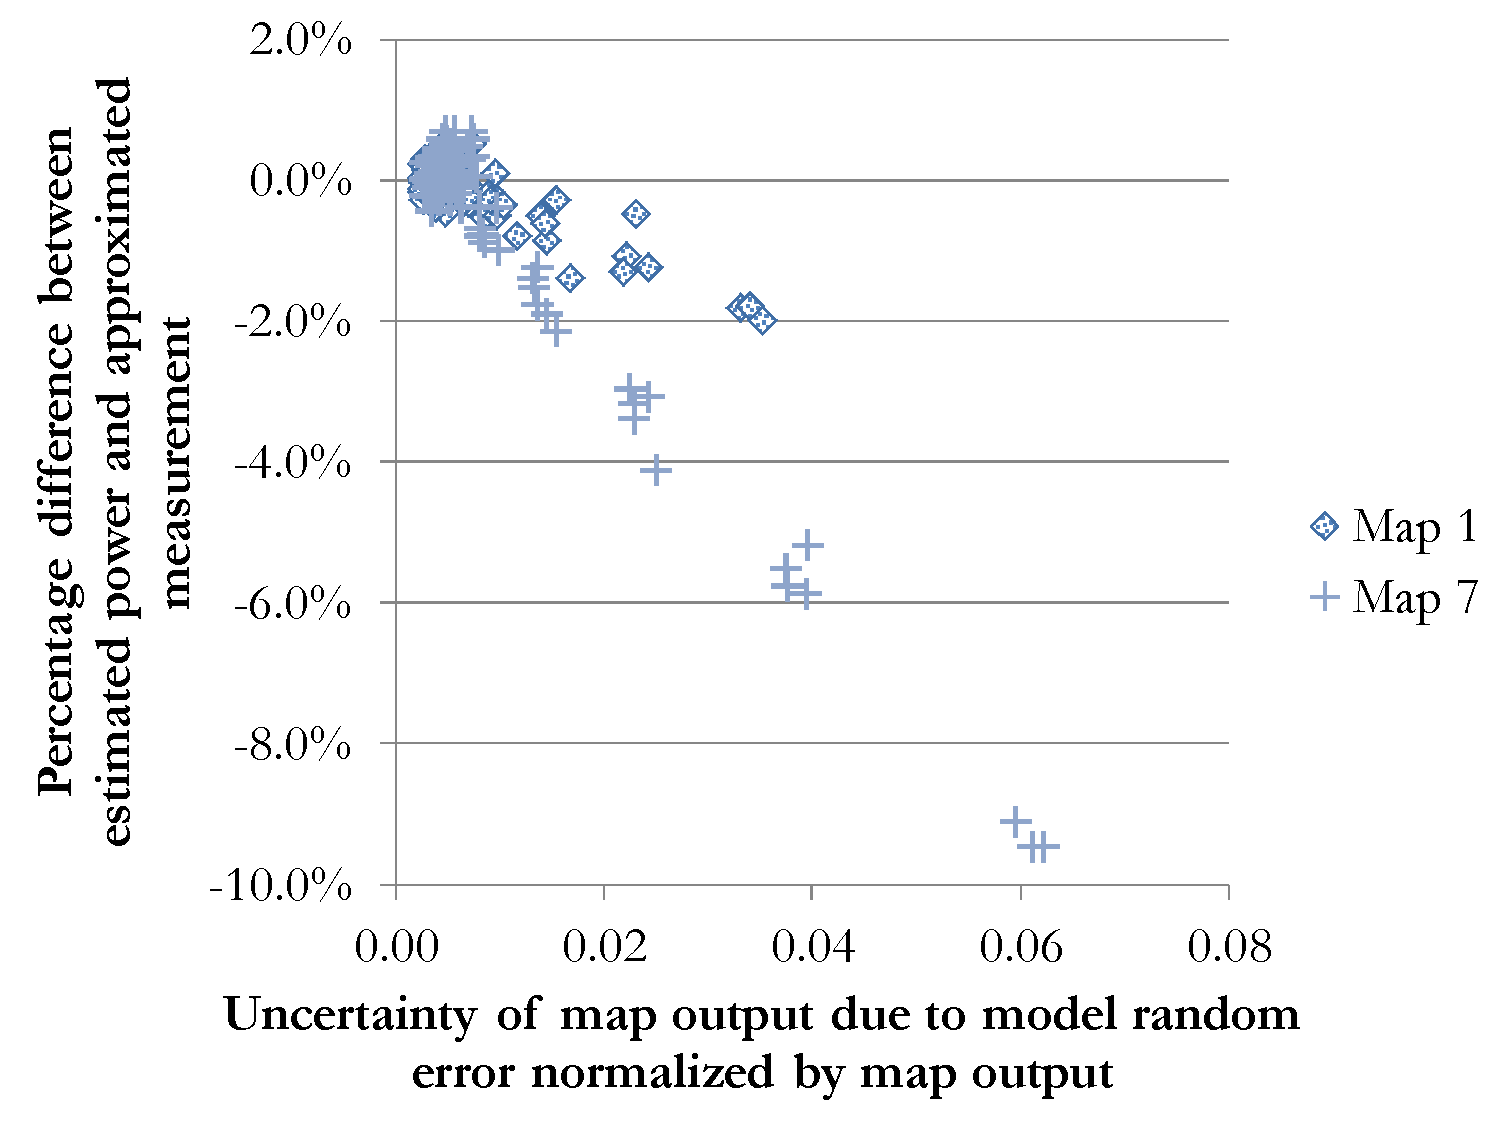
\includegraphics[width=15pc]{num_train_model.pdf}
\caption{\label{fig:num_train_model}Change of accuracy of maps with uncertainty from model random error in Maps 1 and 7.}
\end{minipage}\hspace{2pc}%
\begin{minipage}{15pc}
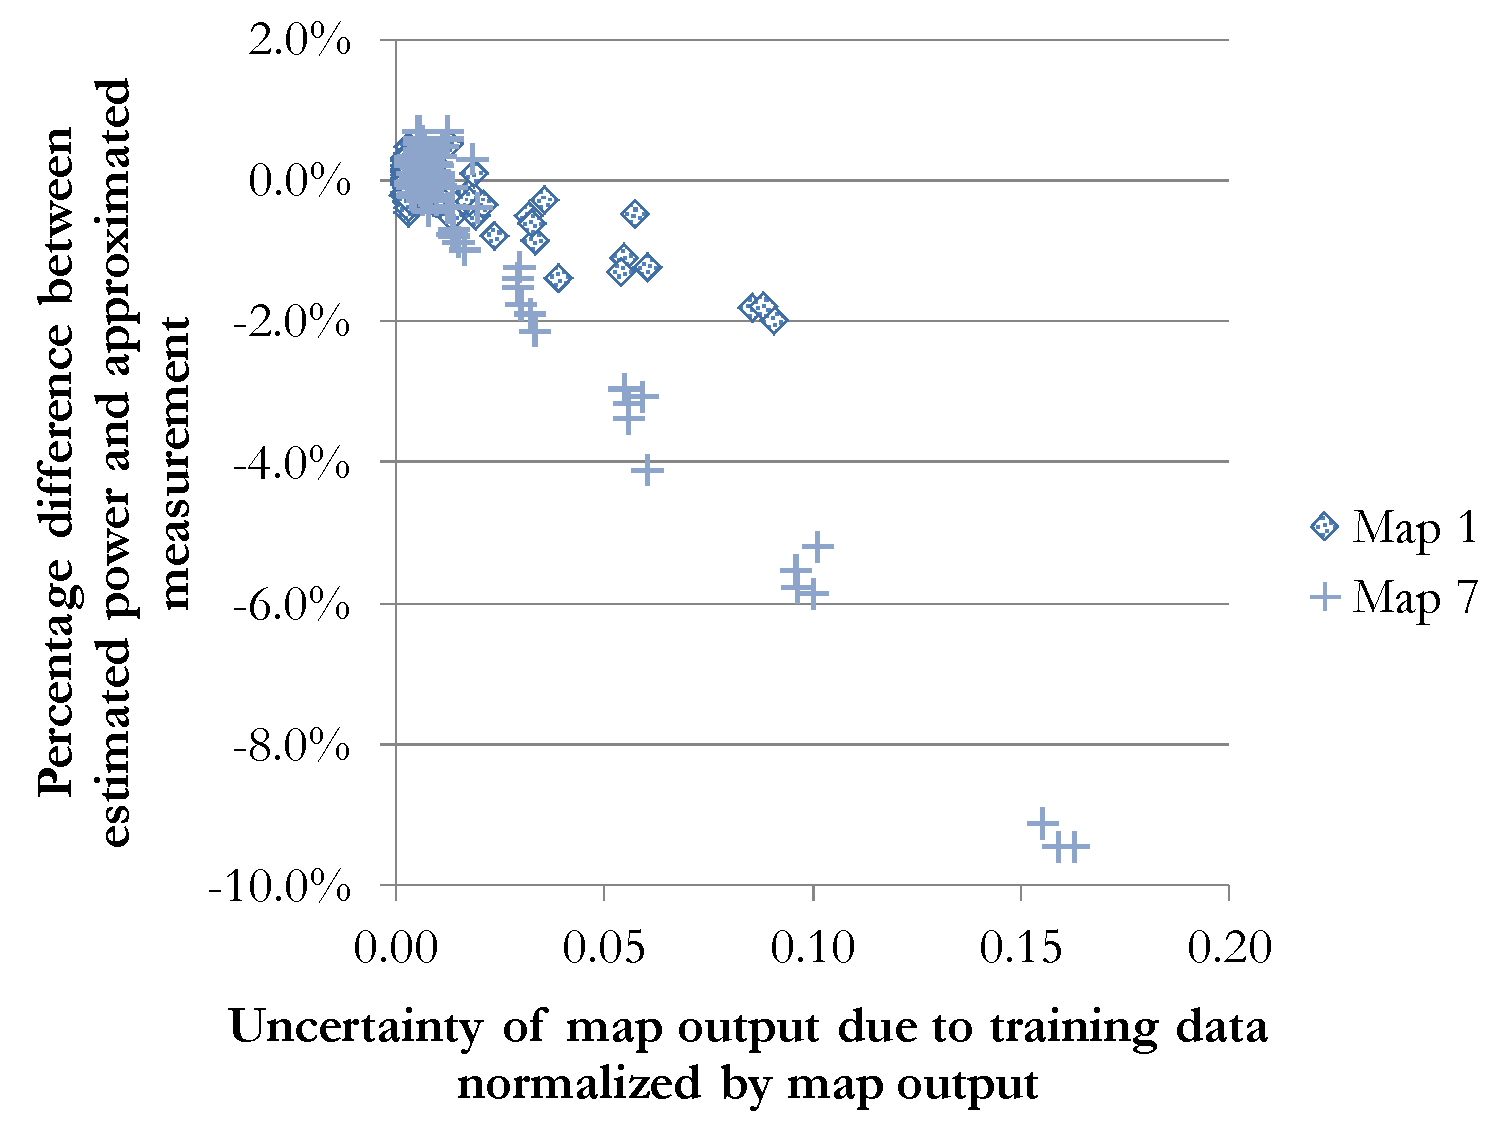
\includegraphics[width=15pc]{num_train_train.pdf}
\caption{\label{fig:num_train_train}Change of accuracy of maps with uncertainty from training data in Maps 1 and 7.}
\end{minipage} 
\end{figure}

Figures \ref{fig:num_train_model} and \ref{fig:num_train_train} show that both the accuracy of Maps 1 and 7 decreases as their uncertainty from model random error and the uncertainty from training data increase, and the reduction of Map 1 accuracy in both figures are more rapid than Map 7. This shows that Map 7, despite having the same training data range as Map 1, is less applicable and accurate as Map 1. This shows that extrapolation uncertainty and accuracy are not only affected by the range of training data but also the number of training data points.\\

The effect of the reduced number of points in the training data is a larger uncertainty for the same distance, e.g. $\sqrt{\Delta T_{cond}^2 + \Delta T_{evap}^2}$, from the nearest training data point as shown in Figure~\ref{fig:map_1_7_unc_C_distance}.  This effect is especially pronounced for large distances (e.g. extrapolated outside training data range of map) of 10\dgC{} or larger and can increase the uncertainty from 10\% (Map 1) to approximately 17\% (Map 7) in the most extreme case.

\begin{figure}[h]
\begin{minipage}{15pc}
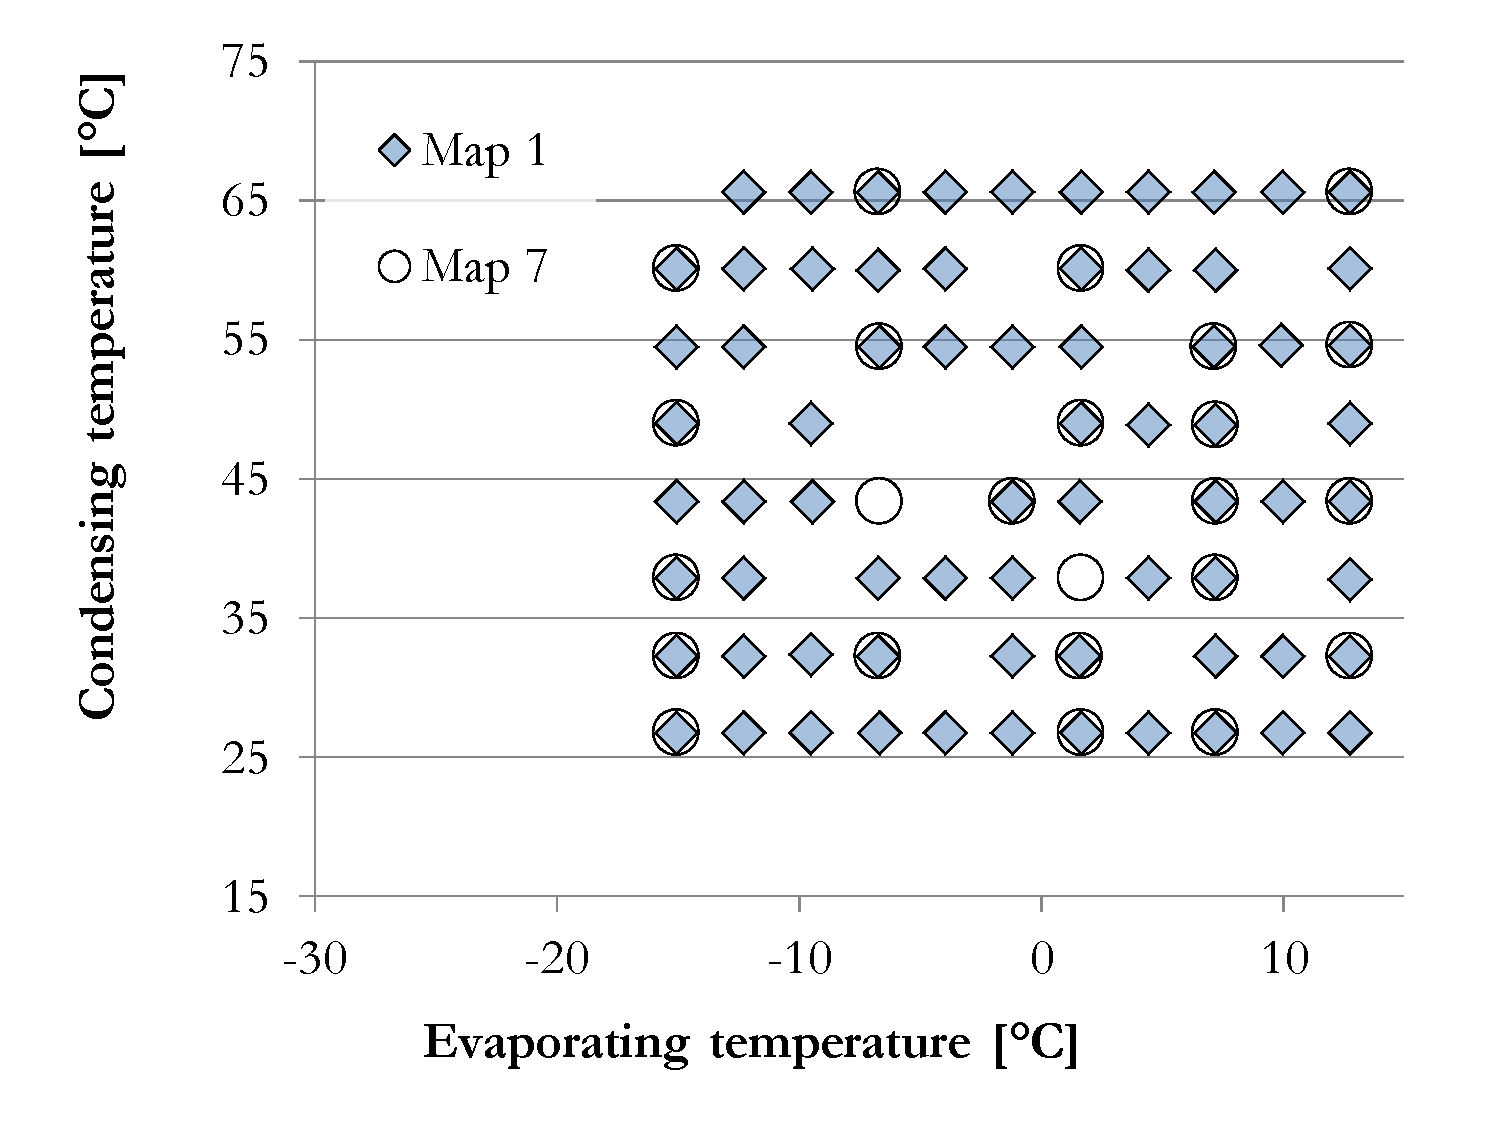
\includegraphics[width=15pc]{./fig/Map_1_and_7_training_data.pdf}
\caption{\label{fig:map_1_7_training_data}Training data points for Maps 1 and 7. Note the absence of low temperature training data.}
\end{minipage}\hspace{2pc}%
\begin{minipage}{15pc}
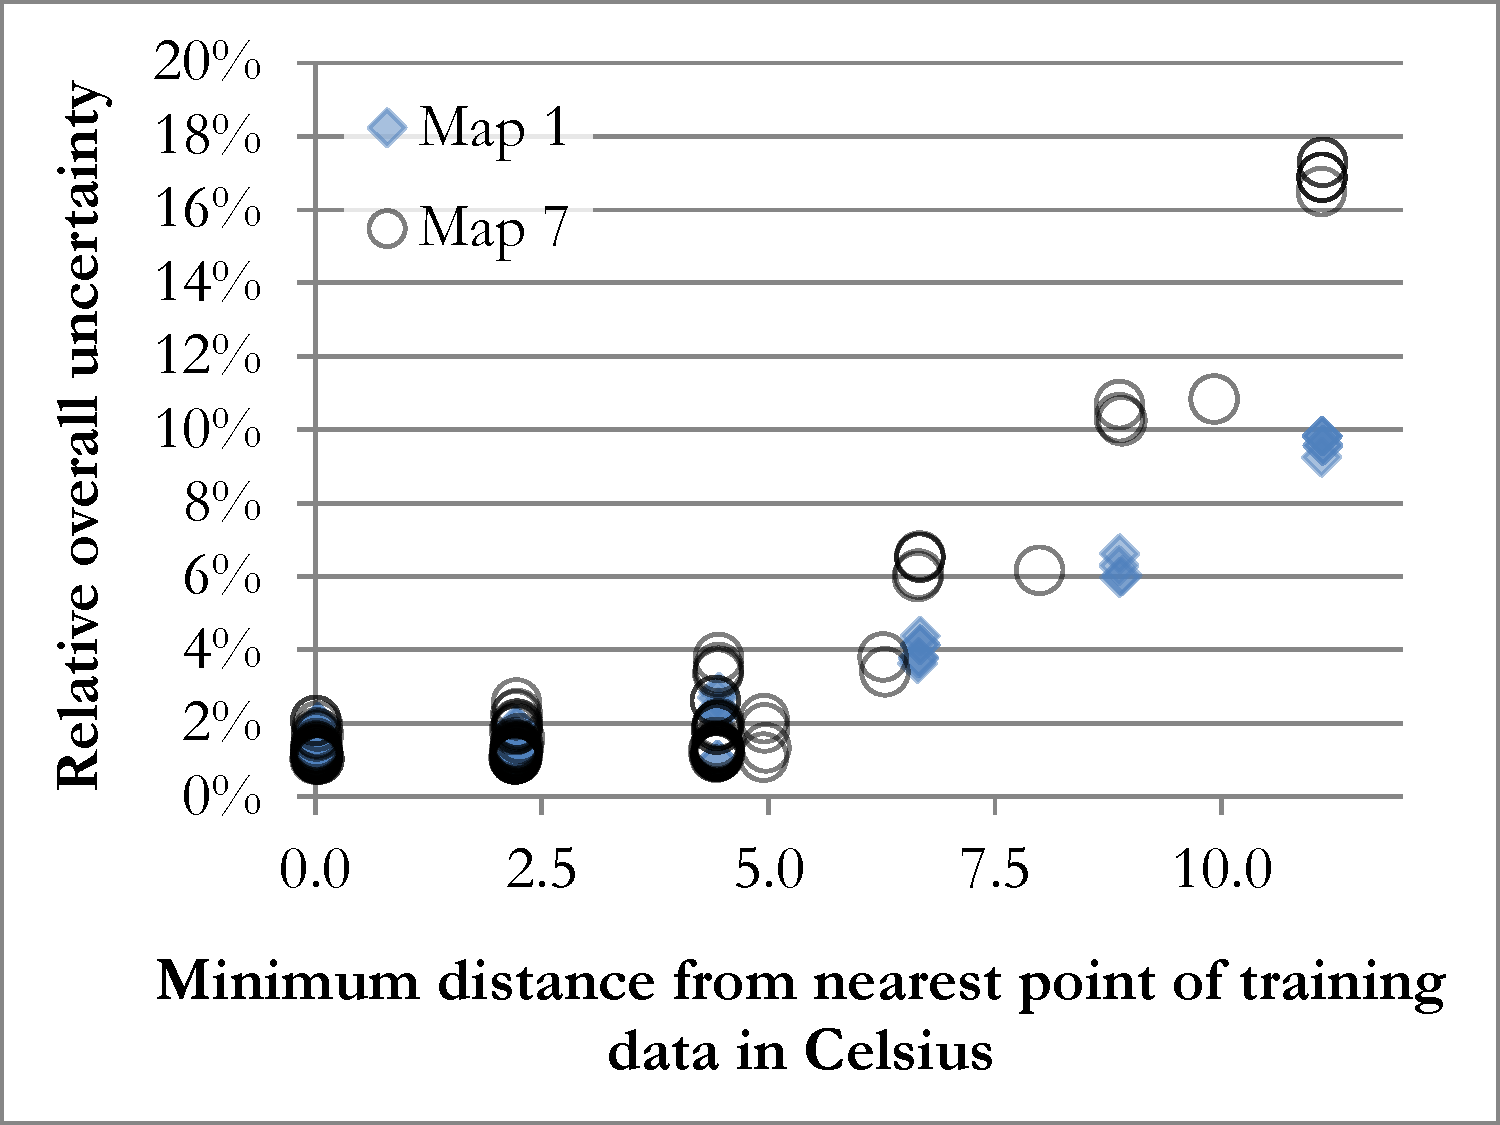
\includegraphics[width=15pc]{./fig/Map_1_and_7_C_distance.pdf}
\caption{\label{fig:map_1_7_unc_C_distance}Change of accuracy with distance to nearest training data point for maps 1 and 7.}
\end{minipage} 
\end{figure}




\section{Conclusions} \label{sec:concl}

To conclude, this paper demonstrates how uncertainty of 10-coefficient compressor maps can be calculated based on the uncertainty due to inputs, the uncertainty due to model random error, the uncertainty due to training data and the uncertainty from outputs. It shows that a method to assess the acuracy and applicability of the map output without measured data outside the training data. It also shows that the range of training data and the number of training data points affect the accuracy and applicability of the map.

\section*{References}
\bibliography{uncer_reference}

\end{document}


